%\documentclass[portrait, a0, plainsections]{sciposter}
\documentclass[11pt]{article}
\usepackage{graphicx}

\begin{document}
	
	\begin{figure}
		\center
		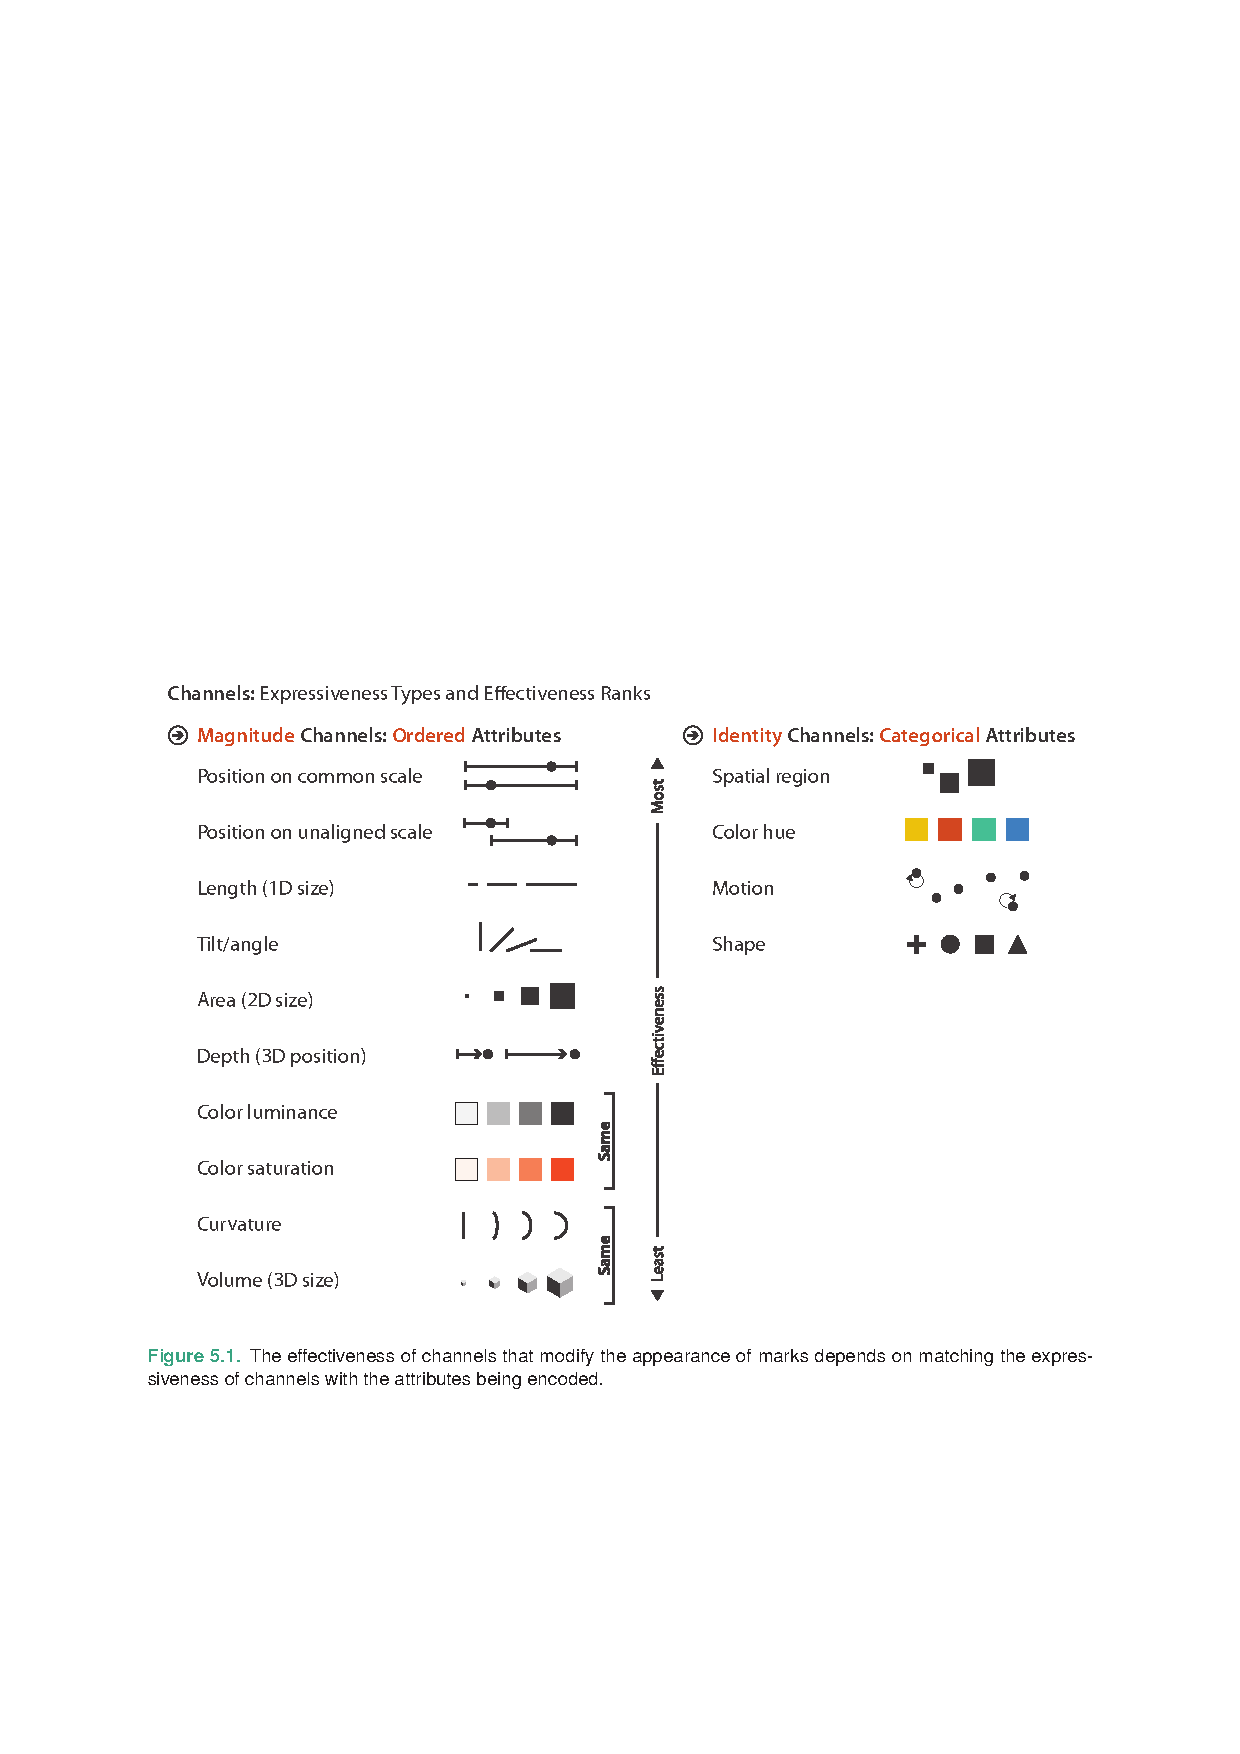
\includegraphics[scale=1,
		trim=80 215 75 330, clip]{channels_marks_effectiveness.pdf}
		\caption{Effectiveness of different channels}
		\label{Fig:efficiency
			}
	\end{figure}
	\paragraph{Marks and Channels\\}
	Marks are the individual elements in a graph, while channels define the appearance of these. Marks can be points in a scatterplot, and the channels could be position on common scale as well as shape. 
	
	Figure \ref{Fig:efficiency} shows the effectiveness of different channels
	
	\paragraph{What-why-how\\}
	Visualizations are made by following the what-why-how principle. What does the data show, and what is the data type are related to "what". The "why" step includes questions such as "Why make the visualization?" and "Consume or produce data?". The last step consists of how to design the visualization, as well as how to create it.
	
	
	
	
\end{document}

